\begin{appendices}

\chapter{Lua Code Snippets}
\label{app:code}

\section{The Runtime Support System}
\label{code:rts}

\begin{listing}[H]
\begin{luacode}
local Event = {}

function Event:new(state_machine_id, event_type, user_data)
	local data = {state_machine_id = state_machine_id, event_type = event_type,
	              user_data = user_data}
	local o = {}

	o.state_machine_id = function ()
		return data.state_machine_id
	end

	o.type = function ()
		return data.event_type
	end

	o.get_data = function ()
		return data.user_data
	end

	o.set_data = function (user_data)
		data.user_data = user_data
	end

	o.timer_id = function ()
		return data.timer_id
	end

	o.set_timer_id = function (timer_id)
		data.timer_id = timer_id
	end

	return o
end

return Event
\end{luacode}
	\caption{Lua code for the event data structure }
	\label{code:event}
\end{listing}

\begin{listing}[H]
\begin{luacode}
local Timer = {}

local function time()
	return os.time()
end

function Timer:new(id, expires, event)
	local data = {id = id, expires = time()+expires, event = event}
	local o = {}

	o.id = function ()
		return data.id
	end

	o.expires = function ()
		return data.expires
	end

	o.event = function ()
		return data.event
	end

	return o
end

return Timer
\end{luacode}
	\caption{Lua code for the timer object }
	\label{code:timer}
\end{listing}

\begin{listing}[H]
\begin{luacode}
local StateMachine = {
	EXECUTE_TRANSITION = 0,
	DISCARD_EVENT = 1,
	TERMINATE_SYSTEM = 2,
}

StateMachine.run = nil

function StateMachine:fire()
	error("'fire' function not yet implemented for this state machine!")
end

function StateMachine:new()
	local o = {}
	setmetatable(o, { __index = self })
	return o
end

return StateMachine
\end{luacode}
	\caption{Lua code for the state machine prototype.}
	\label{code:stm}
\end{listing}

\begin{listing}[H]
\begin{luacode}
local StateMachine = require "stm"

local Scheduler = {}

local function timers_cmp(t1, t2)
	if t1.expires() < t2.expires() then return true end
end

local function time()
	return os.time()
end

function Scheduler:new()
	local o = {}
	setmetatable(o, { __index = self })
	local state_machine_list = {}
	local event_queue = {}
	local timer_queue = {}
	local active_event

	o.time = function ()
		return time()
	end

	o.add_state_machine = function (state_machine)
		state_machine.run = coroutine.create(state_machine.fire)
		state_machine_list[state_machine.id()] = state_machine
		print("State machine '"..state_machine.id().."' added to scheduler.")
	end

	o.get_state_machine = function (id)
		return state_machine_list[id]
	end

	o.remove_state_machine = function (id)
		if state_machine_list[id] then
			result = true
			print("State machine '"..id.."' removed from scheduler.")
		end
		state_machine_list[id] = nil
		return result
	end

	o.add_event = function (event)
		table.insert(event_queue, event)
	end

	o.check_events = function ()
		if event_queue[1] then return true
		else return false end
	end

	o.get_next_event = function ()
		return table.remove(event_queue, 1)
	end

	o.add_timer = function (timer)
		if timer.expires() then
			table.insert(timer_queue, timer)
			table.sort(timer_queue, timers_cmp)
		end
	end

	o.stop_timer = function (id)
		for k, v in pairs(timers) do
			if v.id() == id then
				table.remove(timers, k)
				break
			end
		end
	end

-- continued on next page
\end{luacode}
	\caption{Lua code for the scheduler}
	\label{code:scheduler}
\end{listing}

\begin{listing}[H]
\begin{luacode}
-- Scheduler code continued

	o.check_timers = function ()
		local now = time()
		if timer_queue[1] then
			if timer_queue[1].expires() < now then return true end
		end
		return false
	end

	o.get_next_timeout = function ()
		local now = time()
		if timer_queue[1] then
			if timer_queue[1].expires() < now then return table.remove(timer_queue, 1) end
		end
	end

	o.set_active_event = function (event)
		active_event = event
	end

	o.get_active_event = function ()
		return active_event
	end

	return o
end

function Scheduler:run()
	print("Scheduler running.")
	local success, status, state_machine

	while(true) do	
		local timer, event
		
		if self.check_timers() then
			timer = self.get_next_timeout()
			state_machine = self.get_state_machine(timer.event().state_machine_id())
			self.set_active_event(timer.event())
			success, status = coroutine.resume(state_machine.run, state_machine)
			if not success then
				print("Success: "..tostring(success)..", status: "..status)
				self.remove_state_machine(state_machine.id())
				break
			elseif status == StateMachine.TERMINATE_SYSTEM then
				break
			end

		elseif self.check_events() then
			event = self.get_next_event()
			state_machine = self.get_state_machine(event.state_machine_id())
			self.set_active_event(event)
			success, status = coroutine.resume(state_machine.run, state_machine)
			if not success then
				print("Success: "..tostring(success)..", status: "..status)
				self.remove_state_machine(state_machine.id())
				break
			elseif status == StateMachine.TERMINATE_SYSTEM then
				break
			end

		end
	end
	print("Terminating system...")
end

return Scheduler
\end{luacode}
\end{listing}

\section{The Traffic Light Controller State Machine}
\label{sec:traffic_light_stm}

\begin{listing}[H]
\begin{luacode}
local StateMachine = require "stm"
local Event = require "event"
local Timer = require "timer"

local STMTrafficLightController = StateMachine:new()

local S0, S1, S2, S3, S4, S5 = "S0", "S1", "S2", "S3", "S4", "S5"
local T1, T2, T3, T4, T5 = "t1", "t2", "t3", "t4", "t5"
local YELLOW_DELAY, PEDESTRIAN_TIME, SAFE_TIME = 3, 10, 1

STMTrafficLightController.events = {
	PEDESTRIAN_BUTTON_PRESSED = 1,
	YELLOW_TIMER_EXPIRED = 2,
	PEDESTRIANS_GO = 3,
	PEDESTRIAN_TIMER_EXPIRED = 4,
	CARS_GO = 5,
}

function STMTrafficLightController:schedule_event(event_type, delay, timer_no)
	local event = Event:new(self.id(), event_type)
	local timer = Timer:new(self.id()..timer_no, delay, event)
	event.set_timer_id(timer_no)
	self.scheduler().add_timer(timer)
end

function STMTrafficLightController:new(id, scheduler)
	local o = {}
	setmetatable(o, { __index = self })
	local data = {id = id, state = S0}
	local sched = scheduler

	o.id = function ()
		return data.id
	end

	o.state = function ()
		return data.state
	end

	o.set_state = function (state)
		data.state = state
	end

	o.scheduler = function ()
		return sched
	end

	scheduler.add_state_machine(o)
	return o
end

function STMTrafficLightController:fire()

	print("Pedestrian light set to red.")
	print("Car light set to green.")

	while(true) do
		local event = self.scheduler().get_active_event()
		local current_state = self.state()

		if current_state == S0 then
			if event.type() == self.events.PEDESTRIAN_BUTTON_PRESSED then
				print("Car light set to yellow.")
				self:schedule_event(self.events.YELLOW_TIMER_EXPIRED, YELLOW_DELAY, T1)
				self.set_state(S1)
				coroutine.yield(StateMachine.EXECUTE_TRANSITION)

			else
				coroutine.yield(StateMachine.DISCARD_EVENT)
			end
		
-- continued on next page
\end{luacode}
	\caption{Lua code for the Traffic Light Controller state machine}
	\label{code:traffic_light}
\end{listing}

\begin{listing}[H]
\begin{luacode}
-- STMTrafficLightController continued

	elseif current_state == S1 then
			if event.type() == self.events.YELLOW_TIMER_EXPIRED
			     and event.timer_id() == T1 then
				print("Car light set to red.")
				self:schedule_event(self.events.PEDESTRIANS_GO, SAFE_TIME, T2)
				self.set_state(S2)
				coroutine.yield(StateMachine.EXECUTE_TRANSITION)

			else
				coroutine.yield(StateMachine.DISCARD_EVENT)
			end

		elseif current_state == S2 then
			if event.type() == self.events.PEDESTRIANS_GO
			     and event.timer_id() == T2 then
				print("Pedestrian light set to green.")
				self:schedule_event(self.events.PEDESTRIAN_TIMER_EXPIRED, PEDESTRIAN_TIME, T3)
				self.set_state(S3)
				coroutine.yield(StateMachine.EXECUTE_TRANSITION)

			else
				coroutine.yield(StateMachine.DISCARD_EVENT)
			end

		elseif current_state == S3 then
			if event.type() == self.events.PEDESTRIAN_TIMER_EXPIRED
			     and event.timer_id() == T3 then
				print("Pedestrian light set to red.")
				self:schedule_event(self.events.CARS_GO, SAFE_TIME, T4)
				self.set_state(S4)
				coroutine.yield(StateMachine.EXECUTE_TRANSITION)

			else
				coroutine.yield(StateMachine.DISCARD_EVENT)
			end

		elseif current_state == S4 then
			if event.type() == self.events.CARS_GO
			     and event.timer_id() == T4 then
				print("Car light set to yellow.")
				self:schedule_event(self.events.YELLOW_TIMER_EXPIRED, YELLOW_DELAY, T5)
				self.set_state(S5)
				coroutine.yield(StateMachine.EXECUTE_TRANSITION)

			else
				coroutine.yield(StateMachine.DISCARD_EVENT)
			end

		elseif current_state == S5 then
			if event.type() == self.events.YELLOW_TIMER_EXPIRED
			     and event.timer_id() == T5 then
				print("Car light set to green.")
				self.set_state(S0)
				coroutine.yield(StateMachine.EXECUTE_TRANSITION)
			
			else
				coroutine.yield(StateMachine.DISCARD_EVENT)
			end

		else
			coroutine.yield(StateMachine.DISCARD_EVENT)
		end
	end
end

return STMTrafficLightController		
\end{luacode}
\end{listing}

\begin{figure}[H]
	\centering
	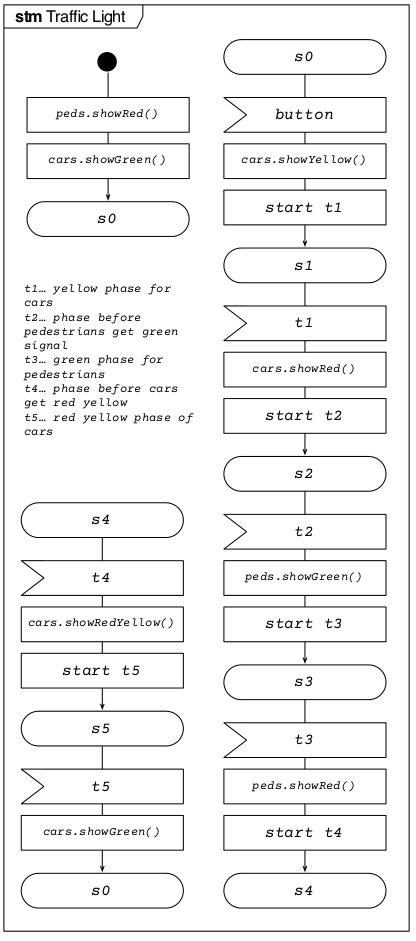
\includegraphics[scale=0.55]{traffic-light-stm}
	\caption[UML specification for Traffic Light Controller]{UML specification for the Traffic Light Controller state machine. Image source: Unit 1 exercise for TTM4160 course, 2013}
	\label{fig:traffic_light_uml}
\end{figure}

\begin{listing}[H]
\begin{luacode}
local Scheduler = require "sched"
local Event = require "event"
local STMTrafficLight = require "stm-light"

local scheduler = Scheduler:new()

local stm_tl1 = STMTrafficLight:new("stm_tl1", scheduler)

local event1 = Event:new(stm_tl1.id(), STMTrafficLight.events.PEDESTRIAN_BUTTON_PRESSED)

scheduler.add_event(event1)
scheduler:run()	
\end{luacode}
	\caption{Lua code for the main program}
	\label{code:main}
\end{listing}

\begin{listing}
\begin{luacode}


\end{luacode}
\end{listing}

\end{appendices}